In this study, two widely used face image datasets were employed: ORL and Extended YaleB. The ORL dataset contains 400 grayscale images from 40 subjects, with each subject having 10 photographs featuring different facial expressions and lighting conditions. The Extended YaleB dataset comprises 2,414 facial images of 38 subjects captured in 9 poses and 64 lighting conditions. To reduce computational complexity, the ORL images were resized from $92 \times 112$ to $30 \times 37$ pixels, while the YaleB images were resized from $168 \times 192$ to $42 \times 48$ pixels, and the pixel values were normalized to scale their range to [0, 1].

On the preprocessed data, we further added salt-and-pepper noise, controlling the noise level and proportion by adjusting the noise parameters $p$ and $r$. Two NMF algorithms were implemented for comparison: the standard $L_2$ NMF and $L_{2,1}$-Norm Based NMF, to evaluate their robustness under different noise conditions. The performance of each algorithm was evaluated using three metrics: Relative Reconstruction Error (RRE), Clustering Accuracy (ACC), and Normalized Mutual Information (NMI).


\subsection{Evaluation Metrics}
To comprehensively evaluate the performance of different NMF algorithms in noisy conditions, this experiment applies three common metrics: Relative Reconstruction Error (RRE), Clustering Accuracy (ACC), and Normalized Mutual Information (NMI). These three metrics evaluate model performance from different perspectives: RRE measures the algorithm's ability to reconstruct the original data, Accuracy reflects the classification consistency of decomposed features in clustering tasks, while NMI quantifies the amount of shared information between the clustering results and the true labels. The combination of these three metrics enables a comprehensive evaluation of the overall performance of the NMF algorithm in terms of reconstruction accuracy and clustering quality, providing a reliable basis for comparing the robustness of different algorithms\cite{sohrabi2025graph}\cite{hedjam2021nmf}.

\subsubsection{Relative Reconstruction Error (RRE)}
The Relative Reconstruction Error (RRE) is used to evaluate how well the reconstructed matrix $WH$ approximates the original clean data $\hat{X}$. It is defined as: 
\begin{align}
    RRE = \frac{\| \hat{X} - WH \|_F}{\| \hat{X} \|_F}
\end{align}
where $\hat{X}$ denotes the clean dataset, and $W$ and $H$ are the basis and coefficient matrices obtained from the NMF decomposition. The smaller the RRE value, the more accurately the algorithm reconstructs the original data, indicating superior stability and robustness. RRE is one of the fundamental metrics for evaluating NMF performance, providing an intuitive reflection of how different algorithms perform in reconstructing data under noisy conditions\cite{sohrabi2025graph}.

\subsubsection{Accuracy (ACC)}
The accuracy of clustering (ACC) is used to evaluate whether the features obtained from NMF decomposition can effectively preserve the class information of the original data. After decomposing $X = WH$, the coefficient matrix $W$ is regarded as the new feature representation. The K-means algorithm is then applied to the columns of $H$, where the number of clusters is set equal to the number of true classes. The accuracy is defined as:
\begin{align}
    Acc(Y, Y_{\text{pred}}) = \frac{1}{n} \sum_{i=1}^{n} \mathbf{1}(Y_{\text{pred}, i} = Y_i)
\end{align}
where $Y$ represents the true labels and $Y_{\text{pred}}$ denotes the predicted labels from clustering. The higher the ACC value, the better the low-dimensional features perform in preserving the class structure. Accuracy is a key metric for evaluating the performance of NMF-based algorithms, reflecting the ability of decomposed features to distinguish between different classes\cite{hedjam2021nmf}.

\subsubsection{Normalized Mutual Information (NMI)}
Normalized Mutual Information (NMI) is used to measure the consistency between the clustering results and the true labels. It evaluates the quality of clustering by calculating the mutual information between the two and normalizing it, defined as follows:
\begin{align}
    NMI(Y, Y_{\text{pred}}) = \frac{2 \times I(Y; Y_{\text{pred}})}{H(Y) + H(Y_{\text{pred}})}
\end{align}
where $I(\cdot)$ denotes the mutual information and $H(\cdot)$ represents the entropy. The NMI value ranges from 0 to 1, with higher values indicating that the clustering results are closer to the true classification structure. Compared to accuracy, NMI is not affected by the permutation of cluster labels and provides a more objective evaluation of clustering performance. NMI is often used in combination with ACC to comprehensively evaluate the performance of NMF algorithms in clustering tasks.

\subsection{Experimental results}

\subsubsection{Relative Reconstruction Error (RRE)}
Relative Reconstruction Error (RRE) is used to measure an algorithm's ability to reconstruct original images in noisy conditions. A smaller value indicates that the model can more accurately restore the original data and possesses greater robustness. In this experiment, we tested both $L_2$-NMF and L$_{2,1}$-NMF on the ORL and YaleB datasets with different combinations of noise parameters $p$ and $r$. The mean and standard deviation of RRE were calculated over multiple runs, and the results are shown in Figure~\ref{fig:RREORL} and Figure~\ref{fig:RRE YaleB}.
\begin{figure}[p]
    \centering
    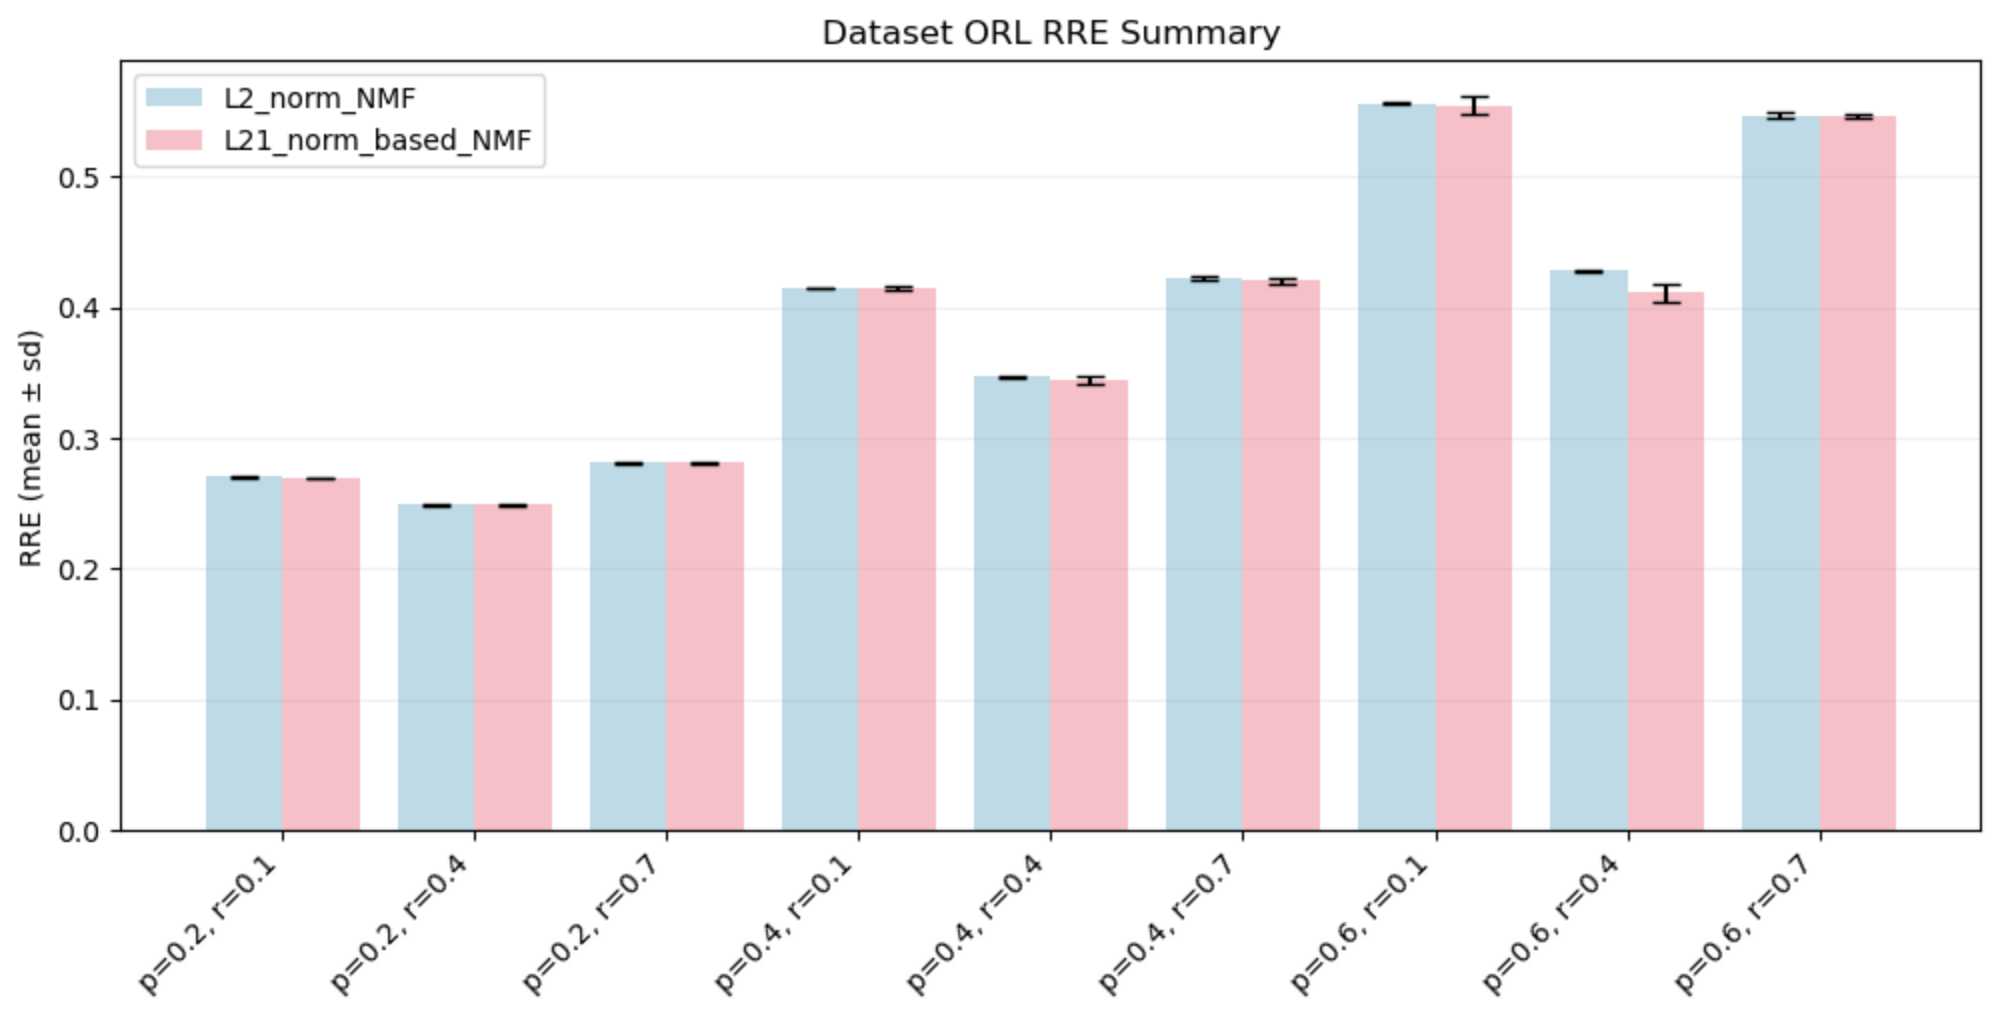
\includegraphics[width=0.9\linewidth]{figure/RRE ORL.png}
    \caption{Dataset ORL RRE Summary}
    \label{fig:RREORL}
\end{figure}

\begin{figure}[p]
    \centering
    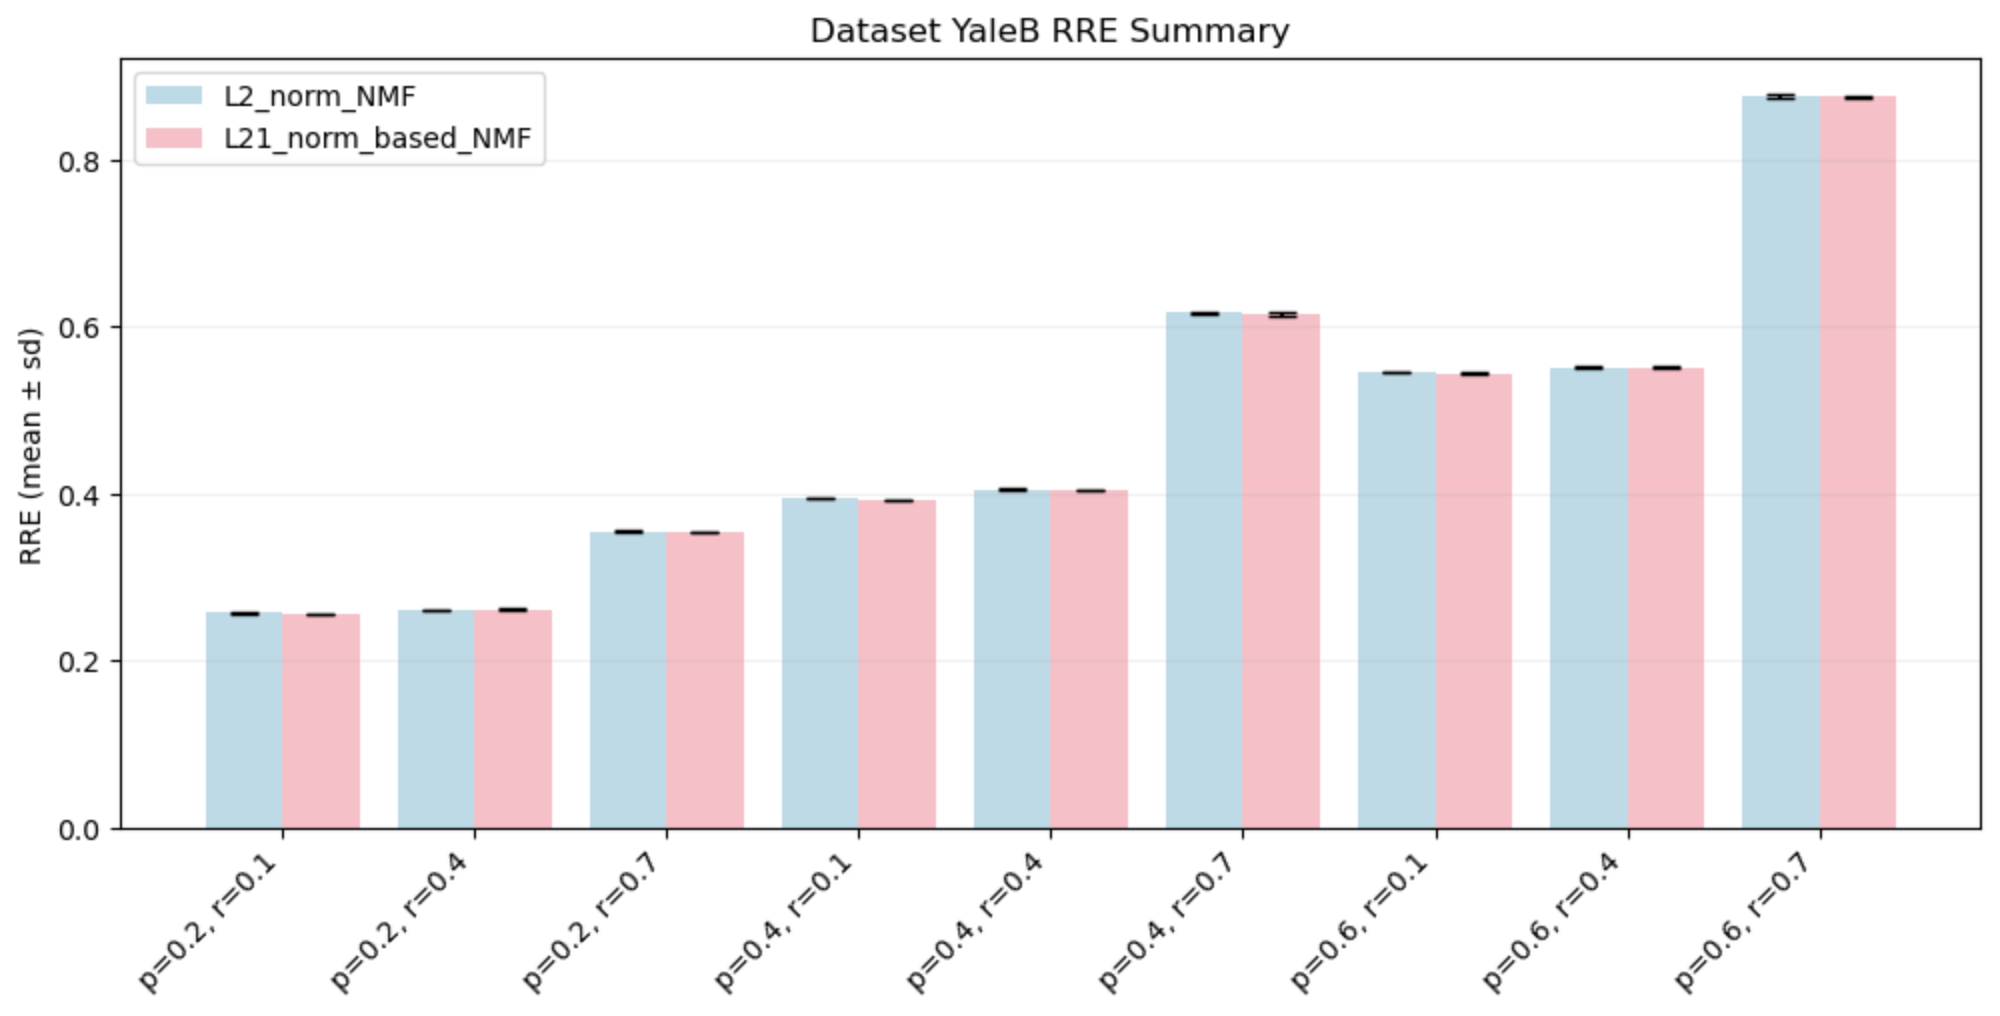
\includegraphics[width=0.9\linewidth]{figure/RRE YaleB.png}
    \caption{Dataset YaleB RRE Summary}
    \label{fig:RRE YaleB}
\end{figure}

The results show that as the noise level $p$ increases, the RRE values across all experiments exhibit a clear upward trend, indicating that higher noise levels significantly decrease the model's reconstruction accuracy. When the white noise proportion $r$ increases, the RRE also rises slightly, showing that white noise tends to have a stronger influence on image reconstruction.

Between the two algorithms, the overall performance is close, but the L$_{2,1}$-NMF shows slightly lower RRE values in most cases. For example, on the ORL dataset when $p=0.4$ and $r=0.4$, the RRE of $L_2$-NMF is 0.3471 while L$_{2,1}$-NMF is 0.3446. The gap becomes larger at higher noise levels, such as $p=0.6$. This result suggests that the L$_{2,1}$-NMF can deal with noisy pixels better and keep more stable reconstruction. The standard deviations are generally small, which means the results are stable and repeatable.

For the  datasets, the ORL dataset exhibits a lower overall RRE due to its smaller sample size and minimal facial conditions, withL$_{2,1}$-NMF having a more visible advantage. The YaleB dataset has more samples and complex lighting conditions, which makes its RRE values higher overall. However, under strong noise (for example $p=0.6$, $r=0.7$), the L$_{2,1}$-NMF still keeps slightly better reconstruction performance. 

In summary, L$_{2,1}$-NMF performs with stronger robustness under conditions of strong noise and non-Gaussian noise, consistent with its theoretical expectation. The detailed RRE results for all parameter settings can be found in Table~\ref{tab:orl_rre} and Table~\ref{tab:yaleb_rre} in the Appendix.

\subsubsection{Accuracy (ACC)}


To further evaluate the clustering performance of both algorithms, we calculated the clustering accuracy (ACC) under different noise settings $(p, r)$. Each experiment was repeated five times, and the mean and standard deviation were recorded.


The accuracy comparison results are shown in Figure~\ref{fig:orl_acc} and Figure~\ref{fig:yaleb_acc}.

\begin{figure}[p]
    \centering
    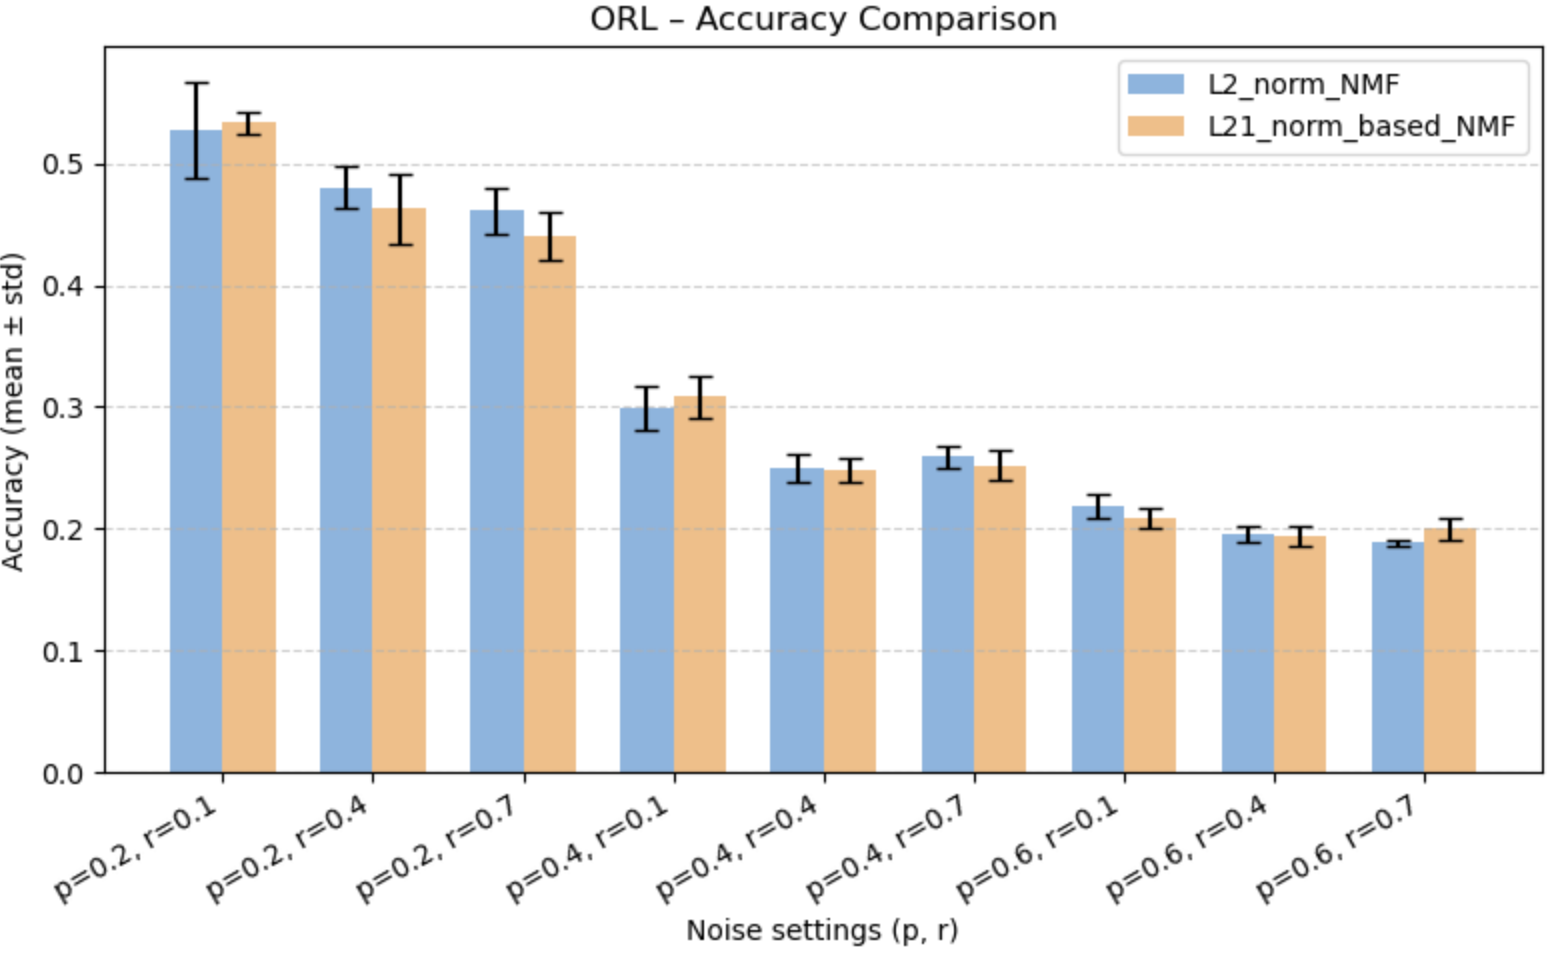
\includegraphics[width=0.9\linewidth]{figure/orl_acc.png}
    \caption{Dataset ORL ACC Summary}
    \label{fig:orl_acc}
\end{figure}

\begin{figure}[p]
    \centering
    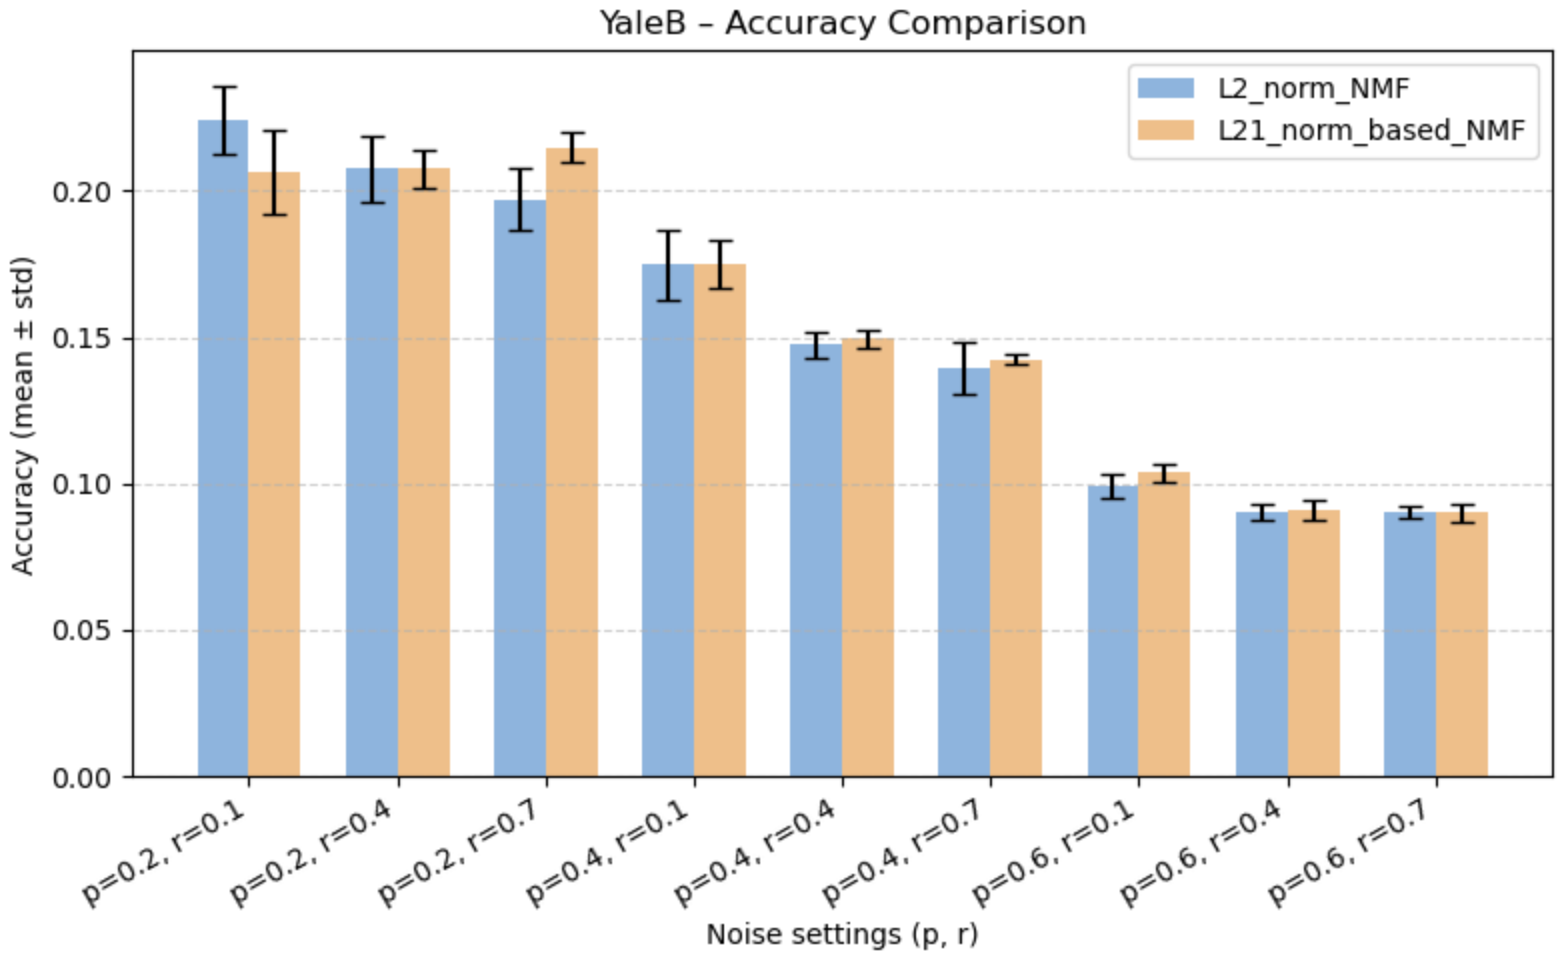
\includegraphics[width=0.9\linewidth]{figure/yaleb_acc.png}
    \caption{Dataset YaleB ACC Summary}
    \label{fig:yaleb_acc}
\end{figure}

The results indicate that as the noise level $p$ increases, the clustering accuracy of both datasets shows a significant downward trend. When $p=0.2, r=0.1$, the average accuracy on the ORL dataset is 0.5278 for $L_2$-NMF and 0.5339 for L$_{2,1}$-NMF. As the noise increases to $p=0.6, r=0.7$, the accuracy drops to 0.1883 and 0.2000 respectively. A similar pattern is observed in the YaleB dataset, where at $p=0.2, r=0.1$, the accuracies of $L_2$-NMF and L$_{2,1}$-NMF are 0.2242 and 0.2065, and they decrease to 0.0903 and 0.0901 when $p=0.6, r=0.7$.
This indicates that increased noise significantly weakens the model's ability to distinguish clusters in the clustering task.

When comparing the two algorithms, L$_{2,1}$-NMF achieves slightly higher accuracy in most cases. For example, on the ORL dataset at $p=0.4, r=0.1$, the accuracy of $L_2$-NMF is 0.2994, while L$_{2,1}$-NMF reaches 0.3083. Under high noise conditions ($p=0.6, r=0.4$), the accuracies are 0.1956 for $L_2$-NMF and 0.1933 for L$_{2,1}$-NMF. Although the difference in accuracy between the two algorithms is small, L$_{2,1}$-NMF is more stable in strong noise conditions and less sensitive to the influence of anomalous pixels.

For the datasets, the ORL dataset achieves higher overall accuracy than YaleB. This is mainly because ORL has fewer samples and minimal facial conditions and lighting conditions. In contrast, the YaleB dataset is significantly affected by lighting, making clustering more challenging and resulting in lower overall accuracy. Nevertheless, both algorithms show similar trends across the two datasets: accuracy decreases as noise increases, and L$_{2,1}$-NMF generally performs slightly better or comparably in most conditions.

The detailed numerical results are listed in Table~\ref{tab:orl_acc} and Table~\ref{tab:yaleb_acc} in the Appendix.

\subsubsection{Normalized Mutual Information (NMI)}
To further evaluate the clustering performance, we calculated the Normalized Mutual Information (NMI), which measures the consistency between clustering results and the true labels. Each experiment was repeated five times, and the mean and standard deviation were recorded. The comparison results are shown in Figure~\ref{fig:orl_nmi} and Figure~\ref{fig:yaleb_nmi}.

\begin{figure}[p]
    \centering
    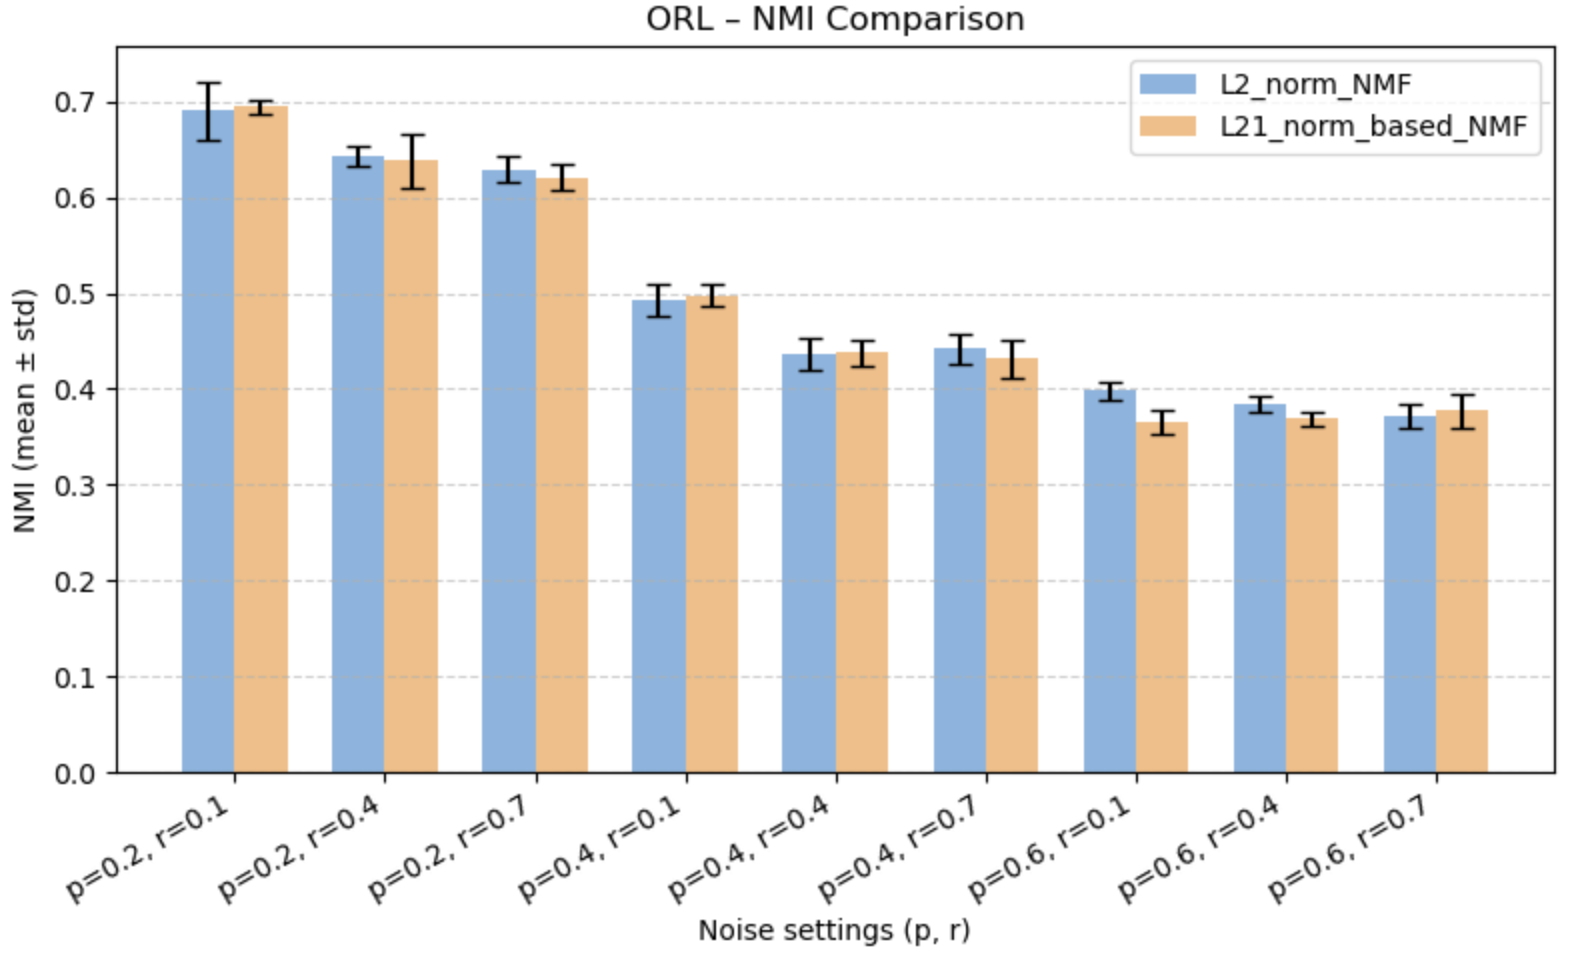
\includegraphics[width=0.9\linewidth]{figure/orl_nmi.png}
    \caption{Dataset ORL NMI Summary}
    \label{fig:orl_nmi}
\end{figure}

\begin{figure}[p]
    \centering
    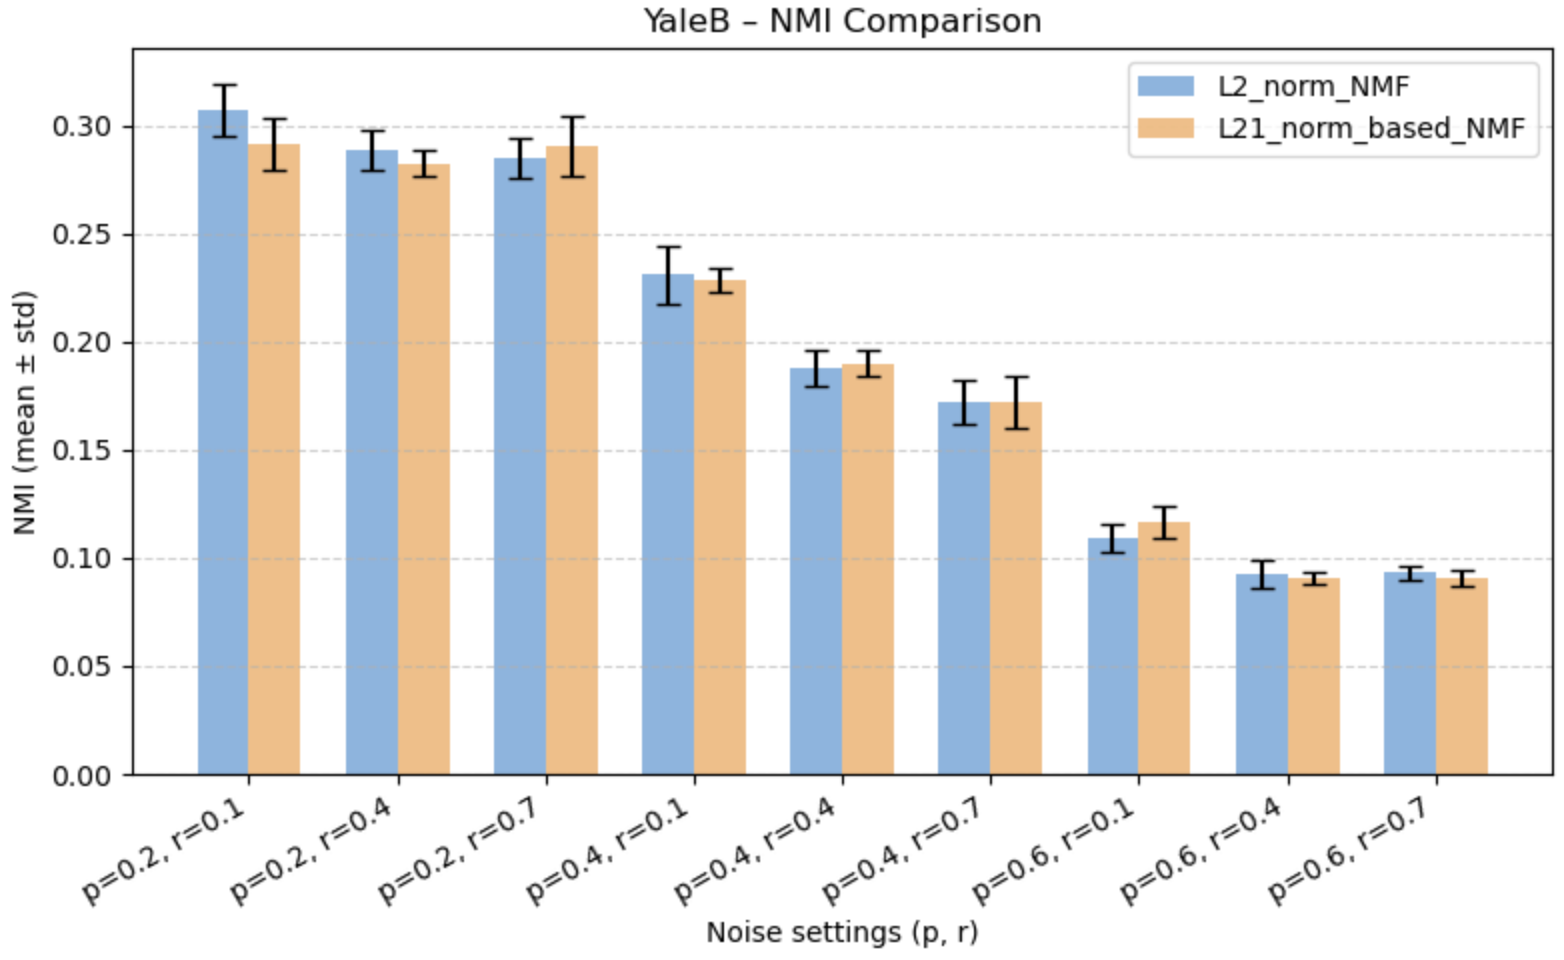
\includegraphics[width=0.9\linewidth]{figure/yaleb_nmi.png}
    \caption{Dataset YaleB NMI Summary}
    \label{fig:yaleb_nmi}
\end{figure}

As seen from the results, the NMI of both algorithms gradually decreases as the noise level $p$ increases. When $p=0.2, r=0.1$, the ORL dataset achieves an NMI of 0.6908 for $L_2$-NMF and 0.6948 for L$_{2,1}$-NMF. When the noise increases to $p=0.6, r=0.7$, the NMI drops to 0.3717 and 0.3769 respectively. A similar trend is observed on the YaleB dataset, where at $p=0.2, r=0.1$, the NMI is 0.3074 for $L_2$-NMF and 0.2910 for L$_{2,1}$-NMF, and decreases to 0.0931 and 0.0905 when $p=0.6, r=0.7$. It can be seen that higher noise levels weaken the correlation between the clustering results and the true labels.

In comparing the algorithms, the NMI value of L$_{2,1}$-NMF is slightly higher than that of $L_2$-NMF in most cases. Although the difference is not significant, it performs more stably in high-noise conditions. For example, on the ORL dataset at $p=0.4, r=0.4$, the NMI values are 0.4366 for $L_2$-NMF and 0.4376 for L$_{2,1}$-NMF; on the YaleB dataset at $p=0.4, r=0.1$, the values are 0.2308 and 0.2282 respectively. The differences are small but stable, indicating that L$_{2,1}$-NMF is more robust.

For the datasets, ORL has a higher overall NMI than YaleB, which is attributed to its smaller sample size and minimal facial conditions and lighting conditions. In contrast, YaleB's large sample size and complex lighting variations make it more challenging for models to preserve inter-class information structures. Overall, increased noise levels lead to a decline in NMI, but L$_{2,1}$-NMF maintains more stable clustering consistency under high noise.

The detailed numerical results are listed in Table~\ref{tab:orl_nmi} and Table~\ref{tab:yaleb_nmi} in the Appendix.